% !TeX root = RJwrapper.tex
\title{\pkg{rmonad}: pipelines you can compute on}
\author{by Zebulun Arendsee, Jennifer Chang, and Eve Syrkin Wurtele}
\maketitle


\abstract{The \CRANpkg{rmonad} package presents a monadic pipeline toolset for
chaining functions into stateful, branching pipelines. As functions in the
pipeline are run, their results are merged into a graph of all past operations.
The resulting structure allows downstream computation on node documentation,
intermediate data, performance stats, and any raised messages, warnings or
errors, as well as the final results. \CRANpkg{rmonad} is a novel approach to
designing reproducible, well-documented, and maintainable workflows in R.}

\section{Background}

% link to pipelining in R
Pipeline programming is common practice in the R community, with
\CRANpkg{magrittr}, \CRANpkg{pipeR}, and \CRANpkg{wrapr} packages offering
infix pipe operators \citep{magrittr2014, pipeR2016, mount2018dot}. The value
on the left of the pipe operator is passed as the first argument to the
right-hand function. This style of programming simplifies code by removing the
need to name intermediate values or write deeply nested function calls. For
example, using the \CRANpkg{magrittr} pipe operator, \code{\%>\%}, the
expression \code{x \%>\% f \%>\% g} is equivalent to \code{g(f(x))}. These
pipelines are equivalent to applied function compositions and termed
function \emph{composition} pipelines.

% introduce general monadic pipelines
A \dfn{monadic} \citep{wadler1990comprehending} pipeline extends composition
pipelines by allowing \emph{context} to be threaded through the pipeline. Each
function call in the pipeline produces both a new value (assuming successful
evaluation) and a computational context surrounding that new value. This new
value and context is then merged with the context of the prior node in the
pipeline, allowing past context to be stored. In this way, monadic pipelines
can be automatically self-describing by returning both the result and a
description of the process that created it.

% introduce rmonad
In this paper, we present \CRANpkg{rmonad}, the first explicitly monadic
pipeline program developed for the R language. \CRANpkg{rmonad} captures the
history of a pipeline as a graph of all past operations. Each node in the graph
represents either an input or a function. These nodes store the source code,
documentation, any raised messages/warnings/errors, benchmarking info, and
arbitrary additional metadata. \CRANpkg{rmonad} also generalizes the standard
linear pipeline to a directed graph with support for branching and looping
pipelines.

% related work: DAG-based workflows
\CRANpkg{rmonad} is one of many graph-based workflow tools available to R
programmers. The \CRANpkg{drake} package \citep{drake} allows specification of
R workflows using Make-family semantics \citep{stallman2002gnu}. The R packages
\CRANpkg{tidycwl} \citep{tidycwl2020} and \CRANpkg{sevenbridges}
\citep{sevenbridges2020} wrap the Common Workflow Language which allows
specification of DAG-based workflows that can be easily run on high-performance
platforms. Many build systems allow execution of R code snippets, such as
Snakemake \citep{koster2012snakemake}, Nextflow \citep{di2017nextflow} and
Cuneiform \citep{brandt2017computation}. Like these programs, \CRANpkg{rmonad}
specifies a graph of dependent operations and can handle large, complex
projects. However, \CRANpkg{rmonad} offers a lighter solution, with no
dependencies outside R.  In the simplest case, \CRANpkg{rmonad} has no more
syntactic complexity than a composition pipeline like \CRANpkg{magrittr}.

% related work: provenance tracking
Since \CRANpkg{rmonad} can annotate and summarize intermediate data, it can
serve as a provenance tracking tool. Provenance tracking of data generated
through a pipeline is critical for research reproducibility
\citep{Gentleman2007StatisticalAA}. For example, the provenance manager
VisTrails builds directed acyclic graphs (DAG) of workflows and stores
intermediate data objects as external XML files in an external database
\citep{Silva2010ProvenanceEnabledDE}. It also provides a visualization of the
workflow (or provenance trail) as it is being run. By visualizing the workflow
in a DAG-like structure, the user can perform exploratory analysis and
retooling on the fly. The R provenance tracking packages \CRANpkg{archivist}
\citep{przemyslaw2017archivist}, \CRANpkg{trackr} \citep{becker2019trackr}, and
\CRANpkg{adapr} \citep{Gelfond2018ASF} store manual annotations (metadata) of
data objects as hooks to an external binary or JSON database.

% tell them what we will tell them
In the following sections, we introduce the \CRANpkg{rmonad} monadic pipeline
operator, show how \CRANpkg{rmonad} generalizes linear pipelines to support branching
and nesting, describe how \CRANpkg{rmonad} evaluation allows pipeline debugging
and annotation, tie these ideas together with a case study, and provide an
overview of the application of \CRANpkg{rmonad} to a large-scale project.

\section{The monadic pipe operator}

A pipeline consists of a series of expressions that are evaluated using
upstream data as input. The context that is passed through an \CRANpkg{rmonad}
pipeline is stored as an ``Rmonad'' S4 object. This object consists of a
directed graph of the relationships between nodes in the pipelines, a list
containing the information about each node (including the output if it is
cached), and a unique identifier for the \dfn{head} node---the node whose
output will be passed to the next operation in the pipeline. Each expression
in the pipeline is evaluated by the special \CRANpkg{rmonad} function,
\code{evalwrap}, that takes an R expression and returns an ``Rmonad'' object.
After each new expression in a pipeline is evaluated, the past ``Rmonad''
object is merged with the new one (see \algref{alg:eval}).

\begin{algorithm}
  \DontPrintSemicolon
  \SetKwFunction{Fmain}{evalwrap}
  \SetKwFunction{Ffailed}{failed}
  \SetKwFunction{FgetMeta}{get\_meta}
  \SetKwFunction{FgetFunction}{get\_function}
  \SetKwFunction{FgetDoc}{get\_doc}
  \SetKwFunction{FgetCodeString}{get\_code\_string}
  \SetKwFunction{FEval}{run}
  \SetKwFunction{Fsuccess}{successful}
  \SetKwFunction{Ftime}{time}
  \SetKwFunction{Fsize}{size}
  \SetKwFunction{FRmonad}{Rmonad}
  \SetKw{Freturn}{return}
  \SetKw{FFALSE}{FALSE}
  \SetKw{FTRUE}{TRUE}
  \SetKw{FNULL}{NULL}
  \SetKw{FNot}{not}
  \SetKwProg{Fn}{function}{:}{}
  \Fn{\Fmain{$x$}}{%
    $metadata$ <- \FgetMeta{$x$} \;
    $doc$ <- \FgetDoc{$x$} \;
    $code$ <- \FgetCodeString{$x$} \;
    $runtime$ <- \texttt{time}(\texttt{\{ }$result$ <- \FEval{$x$} \texttt{\}}) \;
    $isOK$ <- \Fsuccess{result} \;
    \If{isOK}{%
      $y$ <- $result\$value$ \;
      $mem$ <- \Fsize{result\$value} \;
    }
    \Else{%
      $y$ <- \FNULL \;
      $mem$ <- 0 \;
    }
    \Freturn{\FRmonad{y, isOK, code, metadata, doc, runtime, mem}} \;
  }
  \caption{Pseudocode for the \CRANpkg{rmonad} eval function, \code{evalwrap}. \code{get\_meta} and \code{get\_doc} are functions that parse the input expression to extract the documentation string and metadata list. \code{get\_code\_string} gets the R code of the function as a string. These three functions rely on the metaprogramming features of R, which allow functions to operate on the code of their inputs. The \code{run} function is like the standard {\tt eval} R function except that it captures error/warning/message output and returns these together with the output value as a list. \code{\$} is used to access a value in a list. \code{successful} returns TRUE if the evaluation raised no error. \code{size} returns the memory footprint of an R object. \code{Rmonad} is a constructor for an ``Rmonad'' object. In summary, \code{evalwrap} evaluates a function call, captures any raised messages, records information about the function and its output, and returns a new ``Rmonad'' object.}
  \label{alg:eval}
\end{algorithm}

The \CRANpkg{rmonad} function \code{evalwrap} evaluates an R expression and returns an ``Rmonad'' object. The
\dfn{type signature} of \code{evalwrap} is:

\begin{equation}
    \text{evalwrap} :: R \rightarrow M\ a
\end{equation}

The \code{evalwrap} function takes the R expression, $R$, and returns $M\ a$,
which is the ``Rmonad'' object $M$ wrapping the value returned from the
evaluation of $R$. On success, the returned value has type $a$. Thus, whereas a
composition pipeline would consist of chained functions of type $a \rightarrow
b$, $b \rightarrow c$, $c \rightarrow d$, etc, an \CRANpkg{rmonad} pipeline
consists of $a \rightarrow M\ b$, $b \rightarrow M\ c$, $c \rightarrow M\ d$.

Each evaluation step in an \CRANpkg{rmonad} pipeline creates a contextualized
object. However, including the context in the output causes a type conflict.
For example, suppose there are functions $f$ and $g$ with types ($a \rightarrow
M\ b$) and ($b \rightarrow M\ c$), respectively.  Function $f$  produces an
output of type $M\ b$, but function $g$ requires an input of type $b$.  This
conflict is resolved through the special evaluation performed within the
monadic pipe operator.

The monadic pipe operator, or the \dfn{bind} operator, has the type signature \citep{wadler1990comprehending}:

\begin{equation}
  bind\ ::
  \underbrace{m\ b}_{\text{output of $f$}} \rightarrow
  \underbrace{(b \rightarrow m\ c)}_{\text{the function $g$}} \rightarrow
  \underbrace{m\ c}_{\text{output of $g$}}
\end{equation}

\noindent
where $m$ is a generic monad. The function \code{bind} takes an input of type
$m\ b$ and the function $g$ of type ($b \rightarrow m\ c$). It returns the
output of $g$ which has type $m\ c$. Many functions of the general type $a
\rightarrow m\ b$ can be chained together using this \code{bind} function.  For
example, the call \code{bind(bind(f(x), g),h)} would chain the contextualized
results of $f$ through $g$ and then $h$. The implementation of the bind
function defines how context from $m\ b$ is passed through the monadic chain to
$m\ c$.

The simplest possible implementation of the \code{bind} function passes no
state and is identical to applied functional composition (e.g., as done in
\CRANpkg{magrittr}):

\begin{algorithm}
  \DontPrintSemicolon
  \SetKwFunction{Fmain}{stateless\_bind}
  \SetKwFunction{FExtract}{extract}
  \SetKwProg{FIf}{if}{:}{}
  \SetKwProg{FElse}{else}{}{}
  \SetKwFunction{FSuccessful}{successful}
  \SetKwProg{Fn}{function}{:}{}
  \Fn{\Fmain{x, g}}{
    \FIf{\FSuccessful{x}}{
        $y$ = \FExtract{x} \;
        $z$ = $g$($y$) \;
        \Return{z} \;
    } \FElse {} {
        \Return{$fail$} \;
    }
  }
  \caption{The bind function for a \emph{composition} pipeline where no context is passed. \code{successful} returns TRUE if the previous operation succeeded. \code{extract} returns the stored value from the monadic wrapper. $g$ operates on the $y$ and returns the wrapped value $z$.}
\label{alg:bind-comp}
\end{algorithm}


The monadic pipeline operator of \CRANpkg{rmonad}, \code{\%>{}>\%}, has the type signature:

\begin{equation}
  \underbrace{M\ a}_{lhs} \rightarrow \underbrace{(a \rightarrow \ b)}_{rhs} \rightarrow \underbrace{M\ b}_{output}
\end{equation}

\noindent
\code{\%>{}>\%} is a binary operator where the left hand side (\code{lhs}) is an
``Rmonad'' object ($M$) wrapping a value of type $a$. The right hand side
(\code{rhs}) is a normal R function that takes an input of type $a$ and, if
successful, returns a value of type $b$. If \code{lhs} stores a failing state
(i.e., a prior node in the pipeline raised an error), then the \code{rhs}
function is not evaluated and the failed state is propagated. Otherwise, the
value is extracted from \code{lhs} and \code{evalwrap} then evaluates the
\code{rhs} function with the \code{lhs} value as its first argument yielding a
new ``Rmonad'' object. Finally, this new object is merged with the prior,
\code{lhs} ``Rmonad'' object.  Merging involves joining the node graphs of the
old and new ``Rmonad'' objects, setting the head of the resulting graph to the
head of the new graph, and removing the value stored in the prior head  (see
\algref{alg:bind}). The ``head'' of a graph is critical  for branching pipelines
(see the Branching and Nesting section).

\begin{algorithm}
  \DontPrintSemicolon
  \SetKwFunction{Fmain}{rmonad\_bind}
  \SetKwFunction{Ffailed}{failed}
  \SetKwFunction{Feval}{evalwrap}
  \SetKwFunction{Fhead}{head}
  \SetKwFunction{Fvalue}{value}
  \SetKwFunction{FsetValue}{set\_value}
  \SetKwFunction{Funion}{union}
  \SetKw{FFALSE}{FALSE}
  \SetKw{Freturn}{return}
  \SetKwProg{Fn}{function}{:}{}
  \Fn{\Fmain{lhs, rhs}}{%
    {\it h} <- \Fhead{lhs} \;
    \If{\Ffailed{\it h}}{%
      \Freturn{\it lhs} \;
    }
    \Else{%
      $r2$ <- \Feval{rhs, \Fvalue{h}} \;
      $r3$ <- \Funion{lhs, r2} \;
      \If{\Ffailed{r2}}{%
        $r3$ <- \FsetValue{r3, \Fvalue{h}} \;
      }
      \Freturn{r3} \;
    }
  }
  \caption{The \code{\%>{}>\%} \code{bind} function. \code{lhs} and \code{rhs} are the left hand side and right hand side of the binary \code{\%>{}>\%} operator, respectively. \code{lhs} is an ``Rmonad'' object, which is a graph of past operations. \code{head} extracts the current node in the graph that is being acted on (the ``Rmonad'' object stores the index of the current head). \code{failed} returns TRUE if the operation stored in its argument raised an error. \code{value} returns the data stored in a node (or in the head node of an ``Rmonad'' object). \code{evalwrap} evaluates an R function and its arguments and returns a singleton ``Rmonad'' object (see \algref{alg:eval}). \code{union} merges two ``Rmonad'' objects, assigning the head of the new object to the head of the second object. Here the second ``Rmonad'' object is a singleton, so we are adding one node to the function graph and making it the new head node. {\tt set\_value} sets the value of the head node in an ``Rmonad'' object. {\tt rmonad\_bind} returns a new ``Rmonad'' object with a new value on success and the old value on failure.}
  \label{alg:bind}
\end{algorithm}

The difference between \code{\%>{}>\%} and a true monadic \code{bind} operator is
that the \code{rhs} of a monadic bind operator is a function ($a \rightarrow M\
b$), whereas the \code{rhs} of \code{\%>{}>\%} is a normal R function. The
\code{\%>{}>\%} operator essentially transforms the \code{rhs} R function into a function
that yields the monadic object. This is carried out within the monadic bind
function through the special evaluation offered by \code{evalwrap}.

While the primary \CRANpkg{rmonad} operator is the monadic pipe operator,
\code{\%>{}>\%}, several additional operators are provided for operating on
``Rmonad'' objects using pipeline syntax (listed in \tabref{tab:operators}).

\begin{table}[htpb]
  \centering
  \begin{tabular}{ll}
    Operator        & Description \\
    \hline
    \code{\%>{}>\%}   & pass \code{lhs} as initial argument of \code{rhs} function \\
    \code{\%v>\%}   & like \code{\%>{}>\%} but caches the \code{lhs} value \\
    \code{\%*>\%}   & pass list of arguments from \code{lhs} to \code{rhs} \\
    \code{\%\_\_\%} & \code{rhs} starts a new chain that preserves \code{lhs} history \\
    \code{\%||\%}   & use \code{rhs} value if \code{lhs} is failing \\
    \code{\%|>\%}   & call \code{rhs} on \code{lhs} if \code{lhs} failed
  \end{tabular}
  \caption{A partial list of the supported operators. \code{lhs} and \code{rhs} refer to the left-hand and right-hand sides of the given binary operator. \code{\%>{}>\%} is the primary monadic chain operator. \code{\%v>\%} is a variant of the monadic chain operator that always caches its input even on a successful run.  The \code{\%*>\%} operator takes a list of ``Rmonad'' objects on the left and feeds the values of each as arguments into the function on the right, linking the history of each input ``Rmonad'' object to the final ``Rmonad'' object. This operator is important in building branching pipelines. The \code{\%\_\_\%} operator is like a semicolon in a programming language, separating independent pipelines but passing on context. The \code{\%||\%} and \code{\%|>\%}, operators are used in error recovery.}
  \label{tab:operators}
\end{table}

The \code{\%>{}>\%} operator by itself can only create linear chains of operations. Mechanisms for lifting this limitation are introduced in the next section.


\section{Branching and Nesting}

In a linear pipeline, the output of each internal function is piped to just one
downstream function. In contrast, \CRANpkg{rmonad} allows branching to be
formed in one of two main ways: 1) the pipeline's head may be reset to an
internal node and the pipeline can continue growing from there or 2) multiple
pipelines may be merged.

The first branching method uses the \code{tag} function to attach a label to
the current head node and the \code{view} function to change the head node to a
previously tagged node. An example of a branched pipeline using these function
is shown in \figref{fig:rmonad-branch}. A node may be associated with one or
more tags.

The second branching method allows multiple pipelines to merged into one. The
most direct merge method uses the \code{\%*>\%} operator to pass the head
value from each ``Rmonad'' object in the left-hand side list as arguments to
the right-hand side function. \CRANpkg{rmonad} also offers a dedicated
\code{loop} function that takes an ``Rmonad'' object containing a list of
values, passes each into monadic function, and connects the histories and final
results of each pipeline into a new ``Rmonad'' node.

The example below demonstrates a loop where nodes where individual elements are
dynamically tagged for later access:

\begin{example}
m <- loop(
  evalwrap(letters[1:3]),
  function(x){ x %>>% paste0("!") %>% tag(c("letters", x)) }
) %*>% paste0
get_value(m, tag="letters")
#> $`letters/c`
#> [1] "c!"
#> 
#> $`letters/b`
#> [1] "b!"
#> 
#> $`letters/a`
#> [1] "a!"
get_value(m, tag="letters/b")[[1]]
#> "b!"
\end{example}

\noindent
The elements of the first argument to the \code{loop} function (the letters
'a', 'b', and 'c') are passed to \code{loop}'s second argument. The second
argument is an anonymous function that adds an exclamation mark to the input and tags the
resulting value. The tags are hierarchical, thus \code{get\_value(m, tag="letters")} returns all values with the initial tag 'letters'. Specific
values can be accessed like files in a path (e.g., "letters/b").

Since \CRANpkg{rmonad} pipelines are branched, there is in general no single
output value of the pipeline. Rather, the data contained in the ``Rmonad'' object
is queried using a family of vectorized getter functions. For example,
\code{get\_value} will return a list containing the value stored in each node
(or \code{NULL} if no value is stored); \code{get\_error} returns a list of all
error messages, \code{get\_warning} returns a list of all warnings,
\code{get\_code} returns a list of all code strings, etc. The code below fails
on the 'sqrt' call and the failing node can be found by searching for code
blocks that were not successfully executed.

\begin{example}
m <- "a" %>>% paste("cat") %>>% sqrt
get_code(m)[!get_OK(m)]
#> [[1]]
#> [1] "sqrt"
\end{example}

\begin{figure}[!htbp]
  \centering
  \begin{tabular}{| r |}
    \hline
    \begin{minipage}{0.95\textwidth}
\vspace{1mm}
\begin{example}
"x" %>>% paste("a") %>>%
         paste("b") %>>%
         log %>% plot(label="value")
\end{example}
    \end{minipage}
    \\
    \begin{minipage}{0.95\textwidth}
    \centering
    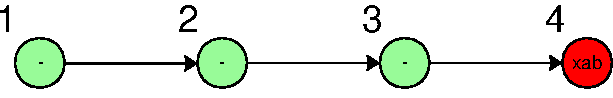
\includegraphics[width=0.5\textwidth]{Images/rmonad_unbranch}
    \end{minipage}
    \\
    \hline
    \begin{minipage}{0.95\textwidth}
\vspace{1mm}
\begin{example}
"x" %>>% paste("a") %>% tag("a1") %>>%
         paste("b") %>>%
         log %>% view("a1") %>>%
         paste("c") %>% plot(label="value")
\end{example}
    \end{minipage}
    \\
    \begin{minipage}{0.95\textwidth}
    \centering
    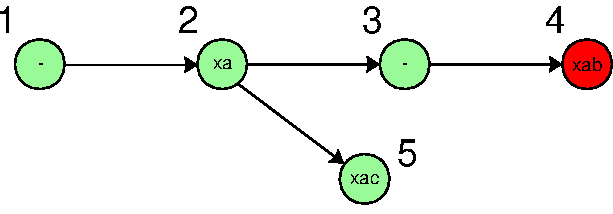
\includegraphics[width=0.5\textwidth]{Images/rmonad_branch}
    \end{minipage}
    \\
    \hline
  \end{tabular}
  \caption{\CRANpkg{rmonad}: linear and branched pipelines. The \code{plot} functions visualize the graph with values in nodes if the values are cached and "-" otherwise. The layout of the plots was modified in the vector editor Inkscape. \textbf{Top:} A linear \CRANpkg{rmonad} pipeline that ends in an error. The pipeline begins at node 1 with the value "x". This is piped into the \code{paste} function which concatenates the letter "a". Since the \code{paste} is successful, the result is stored in node 2 and the value in node 1 is deleted to save memory. The value in node 2 is piped into \code{paste} again, concatenating the letter "b" and storing it in node 3. The value in node 3 is piped into the \code{log} function, where an error is raised, terminating this branch, and storing the final failing value, "x a b", and the error message. The value is only stored at the end node to avoid storing all intermediate values across a pipeline. That way, values are stored when there are errors or where explicitly tagged by the user.  \textbf{Bottom:} A branched \CRANpkg{rmonad} pipeline and its resulting graph. From node 2, the ``Rmonad'' object is piped into the \code{tag} function which annotates the head node (node 2) with the tag "a1" and sets a flag that ensures the value will be cached for later use.  After function 4, the ``Rmonad'' object is piped into \code{view}, which sets the head of the graph to node 2. Lastly, the value in node 2 is piped into the final \code{paste} function that concatenates "c".}
  \label{fig:rmonad-branch}
\end{figure}


In addition to branching, \CRANpkg{rmonad} allows complex pipelines to be built
from smaller nested pipelines defined in normal R functions (see
\figref{fig:rmonad-nest}). When data is piped into a function that wraps a
nested \CRANpkg{rmonad} pipeline, the input values will be linked to the nodes
in the nested pipeline that use the input. In this way, \CRANpkg{rmonad} enables
multilevel debugging. Storing the input to each failed function at each
nest level allows a programmer to step through the code in
the failed node using the input data, without having to rerun the entire
pipeline.

\begin{figure}[!htbp]
  \centering
  \begin{tabular}{| r |}
    \hline
    \begin{minipage}{0.95\textwidth}
\vspace{1mm}
\begin{example}   
# Level 2
f <- function(x) {
  "<" %v>% paste(x) %v>% paste(">")
}
# Level 1
"A" %v>% paste("B")
    %v>% f
    %v>% paste("C") %>% plot(label="value")
\end{example}
    \end{minipage}
    \\
    \begin{minipage}{0.95\textwidth}
    \centering
    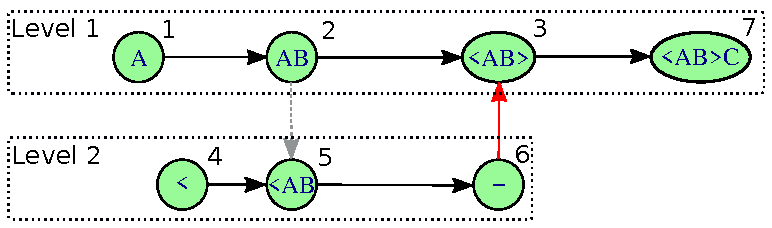
\includegraphics[width=0.7\textwidth]{Images/rmonad_nest}
    \end{minipage}
    \\
    \hline
  \end{tabular}
  \caption{\CRANpkg{rmonad}: complex  pipelines  can  be  built  from  smaller  nested pipelines. Level 1 is a pipeline where the node 3 represents the computation performed by the pipeline in Level 2. The nodes contains values ("A", "AB", etc) if the value is cached by \CRANpkg{rmonad} and contains a "-" if the value is not stored. Arrows show relationships between the nodes. A \textbf{black} arrow shows data being passed directly to a new function. A \textbf{Gray} arrow points from a node in a parent pipeline to a node in a child pipeline that uses its value. The \textbf{red} arrow points from the terminal node in a child pipeline to the node in the parent pipeline that stores its result. Stepping through the pipeline: Node 1 wraps the character "A", node 2 appends "B", and node 3 passes "AB" to the function \code{f}. Next, within the scope of \code{f}, node 4 starts a new pipeline with the value "<", node 5 pastes "<" from node 4 to the local $x$ variable (which is the value passed from node 2), and finally node 6 appends the closing ">" character. The function \code{f} returns an ``Rmonad'' object to node 3. The value of node 6 is transferred to node 3 (thus node 6 is empty, "-"). Finally, node 7 appends "C" and the pipeline finishes successfully.}
  \label{fig:rmonad-nest}
\end{figure}


\section{Evaluation: error handling, metadata, and post-processing}

In this section, we expound on how errors are handled in \CRANpkg{rmonad}, how nodes are documented and annotated, and how post-processing functionality is added to specify log messages, summarize node output and clean up raised messages.

\subsection{Exception handling and tracebacks}

The core functionality of \CRANpkg{rmonad} is the stateful data piping provided
by the monadic operator \code{\%>{}>\%}.  Linear chains of operations can be
constructed with this operator, where each successful node stores information
about the function and results. In the case of an error, \CRANpkg{rmonad}
provides access to the traceback and to the inputs to each failing function.
Knowing the error messages and the function inputs allows the programmer to
step through the failed function and easily diagnose the problem. All
information is stored within the ``Rmonad'' object, rather than in the ephemeral
state of an R session.

Here is a concrete example:

\begin{example}
m <- "a cat" %>>% log %>>% sqrt
get_error(m)
#> [[1]]
#> character(0)
#> 
#> [[2]]
#> [1] "non-numeric argument to mathematical function"
get_code(m)[[2]]
#> "log"
get_value(m)[[2]]
#> [1] "a cat"
\end{example}

\noindent

Here an illegal value is passed into the natural log function. \CRANpkg{rmonad}
catches this error and saves the first failing input and error message. The
node index and error message of the failing function can be found with
\code{get\_error(m)}, the failing expression can be accessed with
\code{get\_code}, and the inputs to the failing function can be retrieved with
\code{get\_value}. This approach scales cleanly to large and deeply nested
pipelines.


\subsection{Parsing code strings, docstrings and metadata lists}

\CRANpkg{rmonad} leverages R non-standard evaluation to parse the abstract
syntax tree of pipeline functions at runtime, prior to evaluation of the
functions. \CRANpkg{rmonad} extracts 1) the function's code as a string, 2) an
optional documentation string, and 3) an optional list of metadata.
All three items are stored in the ``Rmonad'' node. For example:
%
\begin{example}
foo <- function(x){
  "This is a docstring"
  list(sysinfo = sessionInfo())
  return(x)
}
\end{example}
%
\noindent
The first two lines in the function body are the docstring and metadata list,
respectively. Each must 1) be of the appropriate type (string and list,
respectively), 2) not be assigned to a variable, and 3) not be the final line
in the function body. Thus \code{foo} is a legal R function that can be used
naturally outside of the \CRANpkg{rmonad} context. The docstring and metadata
would be ``dead'' lines of code that are evaluated but that are not assigned to
any variable or returned. When \CRANpkg{rmonad} parses the function before
evaluation, the first two lines will be removed and stored, yielding the following
function for evaluation:
%
\begin{example}
function(x){
  return(x)
}
\end{example}

The docstring and the function code are stored as simple strings. The metadata
list is evaluated within the function environment, giving it access to function
input, and then stored.

The metadata is any list associated with a node. It can be used to
store static data such as the author's name, a version for the function,
arbitrary notes. It can also store report generation parameters (like code
chunks in \CRANpkg{knitr}) \citep{knitr}. Because the list is evaluated, its
contents are dynamic, allowing, for example, session info to be stored or
\CRANpkg{knitr} parameters to be a function of the input. Whereas
\CRANpkg{knitr} nests code chunks and their parameters in a text document,
\CRANpkg{rmonad} nests text and parameters within the code.

The metadata can be modified freely even \emph{after} the pipeline is run, to
enable the user to store notes that are a function of the pipeline results, as well as
personal annotations, reminders, or comments on the results.


\subsection{Post-processing functions: formatting, summarizing, and logging}

A built-in use of the metadata is to add formatters, summarizers, and loggers,
which are executed automatically after a node is run. For example, a pipeline
developer might write the following wrapper around a base 10 log function:

\begin{example}
fancy_log10 <- function(x){
  list(
    format_warnings = function(x, xs) {
      sprintf("%s NaNs produced", sum(is.na(x)))
    },
    format_log = function(x, passing) {
      if(passing){
        cat("pass\n")
      } else {
        cat("fail\n")
      }
    },
    summarize = list(len = length)
  )
  log10(x)
}
\end{example}

When run, the captured warnings are processed by \code{format\_warnings} and log messages by \code{format\_log}, with the following result:

\begin{example}
"a cat" %>>% fancy_log10 -> m
#> fail
c(-2,-1,0,1,2) %>>% fancy_log10 -> m
#> pass 
get_warnings(m)
#> [[1]]
#> character(0)
#>
#> [[2]]
#> [1] "2 NaNs produced"
> get_summary(m)[[2]]$len
#> 5
\end{example}

In the first case, an illegal value is passed to the \code{fancy\_log10}
function.  This leads to a failure in the second node, and the logger prints
``fail''. In the second case, the user passes the integers between -2 and 2,
storing the result in \code{m}.  Since these are legal values (from R's
perspective), the logger prints the message ``pass'' after evaluation. When the
returned object is printed, the post-processed warning message ``2 NaNs
produced'' is shown. The result of the summarizing function is accessed through
the \code{get\_summary} function.


\section{Case Study: the Iris data}

As an example of a simple branching \CRANpkg{rmonad} pipeline with error,
warning and run time handling we analyzed the Iris dataset
\citep{anderson1936species, fisher1936use}.  The Iris dataset is often used for
case studies of statistics and machine learning workflows, and consists of
features of three species of flowers: \textit{Iris~setosa},
\textit{Iris~virginia}, and \textit{Iris~versicolor}.  Among these features is
petal length. We used three statistical methods, (1) ANOVA, (2) Kruskal-Wallis,
and (3) t-test, to determine if petal length is significantly different across
the three \textit{Iris} species.  Some statistical methods are not appropriate
for this dataset without data pre-processing. This case study provides an
example of running multiple methods using a branching \CRANpkg{rmonad}
pipeline, while comparing the output and running times of each method.

Normally, a programmer would run the three methods separately using an R script similar to the following:

\begin{example}
# === Load data
data(iris)

# === 3 Statistical Tests (run one at a time)
# (1) Anova
res.aov <- aov(Petal.Length ~ Species, data = iris)
summary(res.aov)

# (2) Kruskal-Wallis
res.kr <- kruskal.test(Petal.Length ~ Species, data = iris)
res.kr

# (3) T-Test
t.test(Petal.Length~Species, data=iris)
\end{example}

Using \CRANpkg{rmonad} tags, data can be branched out to encompass the three
statistical tests. Here, the R variable $m$ stores the output ``Rmonad'' S4
object. We must initially tag the branch point node (in this case, the original
Iris dataset). Since we gave the first node the tag (``indata''), its
value will be cached and can be accessed with the command \code{get\_value(m,
tag="indata")}. From here, we can access and pipe (\code{\%>{}>\%}) the viewed
``indata'' tag into the different statistical tests, as scripted below and
visualized in \textbf{Figure 3}.

\begin{example}
# === rmonad (run together)
m <- {
  "iris dataset"
  evalwrap(iris, tag="indata")
} %>>% {
  "anova"
  res.aov <- aov(Petal.Length ~ Species, data = .)
  summary(res.aov)
} 

m <- {
  view(m, "indata")
} %>>% {
  "Kruskal-Wallis"
  res.kr <- kruskal.test(Petal.Length ~ Species, data = iris)
  res.kr
}

m <- {
  view(m, "indata")
} %>>% {
  "t-test"
  t.test(Petal.Length~Species, data=iris)
}
\end{example}

The above code could have been chained together using \code{\%>\%
get\_value(tag="indata") \%>\%} commands, but instead was separately added to the $m$
rmonad object for ease of reading. From the $m$ rmonad objects, we can plot the
pipeline. In the following command we label the nodes by node id,
documentation, running time, and any errors if they exists.

\begin{example}
plot(m, label = function(m){paste(get_id(m),
                                  get_doc(m), 
                                  get_time(m),
                                  gsub("character\\(0\\)", "", get_error(m)), 
                                  sep=":")})
\end{example}

\begin{figure}[htbp]
  \centering
  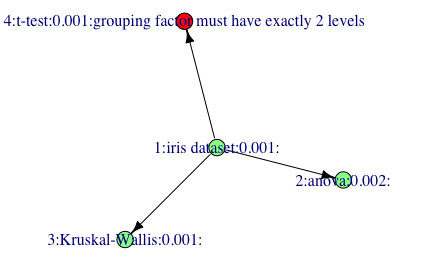
\includegraphics[width=0.6\textwidth]{Images/rmonad_threetests}
  \caption{Using \CRANpkg{rmonad} for three statistical tests. The Iris dataset is piped to (1) ANOVA, (2) Kruskul-Wallis, and (3) t-test. Node color reflects whether the test ran (green) or threw an error (red). Time in seconds is shown next to the test name. Errors are annotated on the node. Notice how t-test has the error: "grouping factor must have exactly 2 levels". Of the two tests without errors, ANOVA ran slightly slower than Kruskal-Wallis.}
  \label{fig:rmonad-irispipeline}
\end{figure}

In \figref{fig:rmonad-irispipeline}, the center node is the iris dataset and
has three arrows going outwards toward one red and two green nodes. Of those,
the red node near the top represents the t-test and shows the expected error
``grouping factor must have exactly 2 levels''. Since we are testing the petal
length among the three species, this error is expected. Any errors of the
pipeline can also be obtained in a table:

\begin{example}
missues(m)
#>   id  type                                      issue
#> 1  4 error grouping factor must have exactly 2 levels
\end{example}

Going clockwise, ANOVA and Kruskal-Wallis are represented by nodes 2 and 3. The
green nodes indicate that both ran although their running times were different.
From their node labels, Kruskal-Wallis ran in 0.001 ms, slightly faster than
ANOVA (0.002). Also note that green nodes only indicate that the method ran
successfully, not the results of that method or statistical significance. The
results of the ANOVA and Kruskal-Wallis test can be pulled out of the pipeline
using their Node ID number and the following commands.

\begin{example}
> id=c(2,3)           # place id(s) of end result(s) here
> get_value(m)[id]
#> [[1]]
#>              Df Sum Sq Mean Sq F value Pr(>F)    
#> Species       2  437.1  218.55    1180 <2e-16 ***
#> Residuals   147   27.2    0.19                   
#> ---
#> Signif. codes:  0 ‘***’ 0.001 ‘**’ 0.01 ‘*’ 0.05 ‘.’ 0.1 ‘ ’ 1
#> 
#> [[2]]
#> 	Kruskal-Wallis rank sum test
#> 
#> data:  Petal.Length by Species
#> Kruskal-Wallis chi-squared = 130.41, df = 2, p-value < 2.2e-16
\end{example}

Both tests agree that there is a significant difference between
\code{Petal.Length} across the three Iris species. ANOVA ran on the dataset,
which means that petal length follows a normal distribution within each
species. Kruskal-Wallis does not assume a normal distribution. The analyst can
decide which method to use; in this case the conclusion is the same.
\figref{fig:rmonad-irispipeline} is an example of a branched \CRANpkg{rmonad}
pipeline comparing three different statistical methods applied to the iris
dataset to test a hypothesis.

\section{\CRANpkg{rmonad} in the wild: a comparative genomics case study}

An example of a large and complex pipeline that uses \CRANpkg{rmonad} is the
orphan gene classification R pipeline, {\tt fagin}
\citep{arendsee2019fagin} (\figref{fig:rmonad-fagin}). This pipeline compares
genes from one species of interest (the focal species) to genomes of several
related species. The first step in the pipeline is to store the user's session
information, which can be used in debugging if needed. Next, the pipeline loops
across each species, where, for each species, genomes and annotation data are
loaded and validated.   Then secondary data (e.g., protein sequences) are
derived, and diagnostic summaries are produced and stored.  Next, each of the
orphan genes in the focal species is compared to each of the related species
genomes to create 12 features that are used to classify potential evolutionary
relatives of each the focal gene in the target species. Finally, all data for
each focal gene is compiled into a description.

The output of this pipeline is a single ``Rmonad'' object. Further analysis
of the pipeline entails a series of queries against this returned object.
Warnings and messages are tabulated into an HTML report. Tagged summary data is
extracted and used to build diagnostic figures. The primary results are
extracted as tabular data and visualized in the final report. Issues with a
pipeline can be identified by searching through the raised warnings stored in
the ``Rmonad'' object. Debugging consists of identifying the node of failure,
extracting the stored inputs to the failing node, and then stepping through the
failing code.

\begin{figure}[htbp]
  \centering
  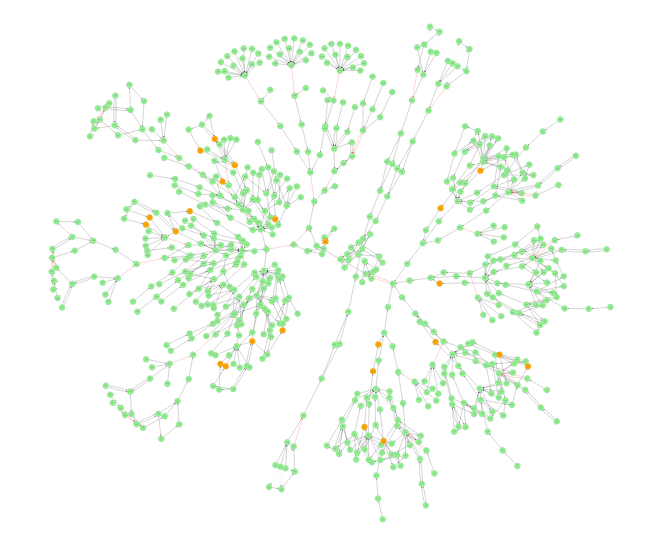
\includegraphics[width=0.8\textwidth]{Images/rmonad_fagin}
  \caption{\CRANpkg{rmonad} can handle large projects. Here,  \CRANpkg{rmonad} analysis of the {\tt fagin} pipeline is shown. Green nodes represent passing; orange nodes raise warnings. The four symmetric subtrees on the right represent a loop that loads and validates the input data for four plant species. The two sets of three symmetric subtrees on the left are loops comparing each of the four species ({\it A.~thaliana}) to the other three.}
  \label{fig:rmonad-fagin}
\end{figure}

\section{Conclusion}

% overview and general motivation
We implemented a monadic pipeline in R via the \CRANpkg{rmonad}
package. \CRANpkg{rmonad} provides an infrastructure for data analysis and
report generation. \CRANpkg{rmonad} stores pipeline results and metadata that
can be easily explored interactively and collated into reports using tools such
as the literate programming package \CRANpkg{knitr} \citep{knitr} or the HTML
report generator \CRANpkg{Nozzle.R1} \citep{gehlenborg2013nozzle}.

\CRANpkg{rmonad} integrates a simple profiler into the workflows by
automatically capturing the runtime and memory usage of each node. This feature
makes it easier for the pipeline developer to identify bottlenecks in the code
or potential culprits of memory overflow. Often, a coder must add benchmarking code to key locations in a pipeline.  \CRANpkg{rmonad} has \textit{built-in} benchmarking, such that all locations in the pipeline are automatically tested and performance can be checked post-run.

% debugging and issue reports
\CRANpkg{rmonad} provides a powerful tool for creating and resolving issue
reports. If an \CRANpkg{rmonad} pipeline fails, the resulting object will store
all failing functions, their raised error/warning messages and also their
inputs. This object can be used to find
the error messages, load all inputs to the failing function, and proceed
to step through the code until the bug is found. If the user prepends a node that
stores the local session data (e.g., \code{{sessionInfo()} \%\_\_\% ...}), the
debugger gains access to the state of the user's machine (an often-requested item in a bug report). An ``Rmonad'' object with session info attached contains everything needed to debug the issue.
This streamlines issue resolution by improving automation and simplifying submission.

% future directions: parallelism and caching (there are more future ideas I
% could include)
Performance has not been a focus of \CRANpkg{rmonad} up to this point. The
package currently lacks support for the re-use of cached values when pipelines
are re-run. Also each evaluation step has a high overhead cost relative to
lighter pipeline tools like \CRANpkg{magrittr}. \CRANpkg{rmonad} pipelines
tend to be memory intensive, since they store many intermediate results and
metadata in the ``Rmonad'' objects. Addressing these performance issues is a
major goal for future work.

% overview
In summary, \CRANpkg{rmonad} integrates the concepts of a pipeline, a build
system, a data structure, and an low-level report-generating engine. An
\CRANpkg{rmonad} project consists of 
incremental piped operations (like
a pipeline program), supports complex branching projects (like a build system),
and produces a data structure that can be computed on to generate dynamic
reports.

\section{Availability}

\CRANpkg{rmonad} is published under the GPL-3 license and is available on the Comprehensive R Archive Network (CRAN) and on GitHub at \url{https://github.com/arendsee/rmonad}. Systematic documentation of the features with simple examples can be found in the vignettes, available through CRAN.


\section{Funding}

This material is based upon work supported by the National Science Foundation
under Grant No. IOS 1546858.

\bibliography{rmonad}

\address{Zebulun Arendsee\\
  Iowa State University \\
  Ames IA, USA \\
  https://orcid.org/0000-0002-5833-798X \\
  \email{zbwrnz@gmail.com}}

\address{Jennifer Chang \\
  Iowa State University \\
  Ames IA, USA \\
  https://orcid.org/0000-0002-8381-3765 \\
  \email{jennifer.chang.bioinform@gmail.com}}
  
\address{Eve Wurtele \\
  Iowa State University \\
  Ames IA, USA \\
  https://orcid.org/0000-0003-1552-9495\\
  \email{eve@iastate.edu}}
